\documentclass[12pt]{article}
\setlength\parindent{0pt}
\usepackage{fullpage}
\usepackage{amsmath}
\usepackage{graphicx}
\setlength{\parskip}{4mm}
\def\LL{\left\langle}   % left angle bracket
\def\RR{\right\rangle}  % right angle bracket
\def\LP{\left(}         % left parenthesis
\def\RP{\right)}        % right parenthesis
\def\LB{\left\{}        % left curly bracket
\def\RB{\right\}}       % right curly bracket
\def\PAR#1#2{ {{\partial #1}\over{\partial #2}} }
\def\PARTWO#1#2{ {{\partial^2 #1}\over{\partial #2}^2} }
\def\PARTWOMIX#1#2#3{ {{\partial^2 #1}\over{\partial #2 \partial #3}} }
\newcommand{\BE}{\begin{displaymath}}
\newcommand{\EE}{\end{displaymath}}
\newcommand{\BNE}{\begin{equation}}
\newcommand{\ENE}{\end{equation}}
\newcommand{\BEA}{\begin{eqnarray}}
\newcommand{\EEA}{\nonumber\end{eqnarray}}
\newcommand{\EL}{\nonumber\\}
\newcommand{\la}[1]{\label{#1}}
\newcommand{\ie}{{\em i.e.\ }}
\newcommand{\eg}{{\em e.\,g.\ }}
\newcommand{\cf}{cf.\ }
\newcommand{\etc}{etc.\ }
\newcommand{\Tr}{{\rm tr}}
\newcommand{\etal}{{\it et al.}}
\newcommand{\OL}[1]{\overline{#1}\ } % overline
\newcommand{\OLL}[1]{\overline{\overline{#1}}\ } % double overline
\newcommand{\OON}{\frac{1}{N}} % "one over N"
\newcommand{\OOX}[1]{\frac{1}{#1}} % "one over X"



\begin{document}
\pagenumbering{gobble}
\Large
\centerline{\sc{Recitation Questions}}
\normalsize
\centerline{\sc{Week of 22 February}}

\begin{minipage}{0.7\textwidth}
Two weights of mass $m_1$ and $m_2$ are attached to either end of a string. This string is passed over a light pulley, as shown in the image.
Clearly the heavier mass will go down and the lighter one will go up, but at what rate? In this problem, you will calculate their acceleration.
\end{minipage} \hfill
\begin{minipage}{0.3\textwidth}
\begin{center}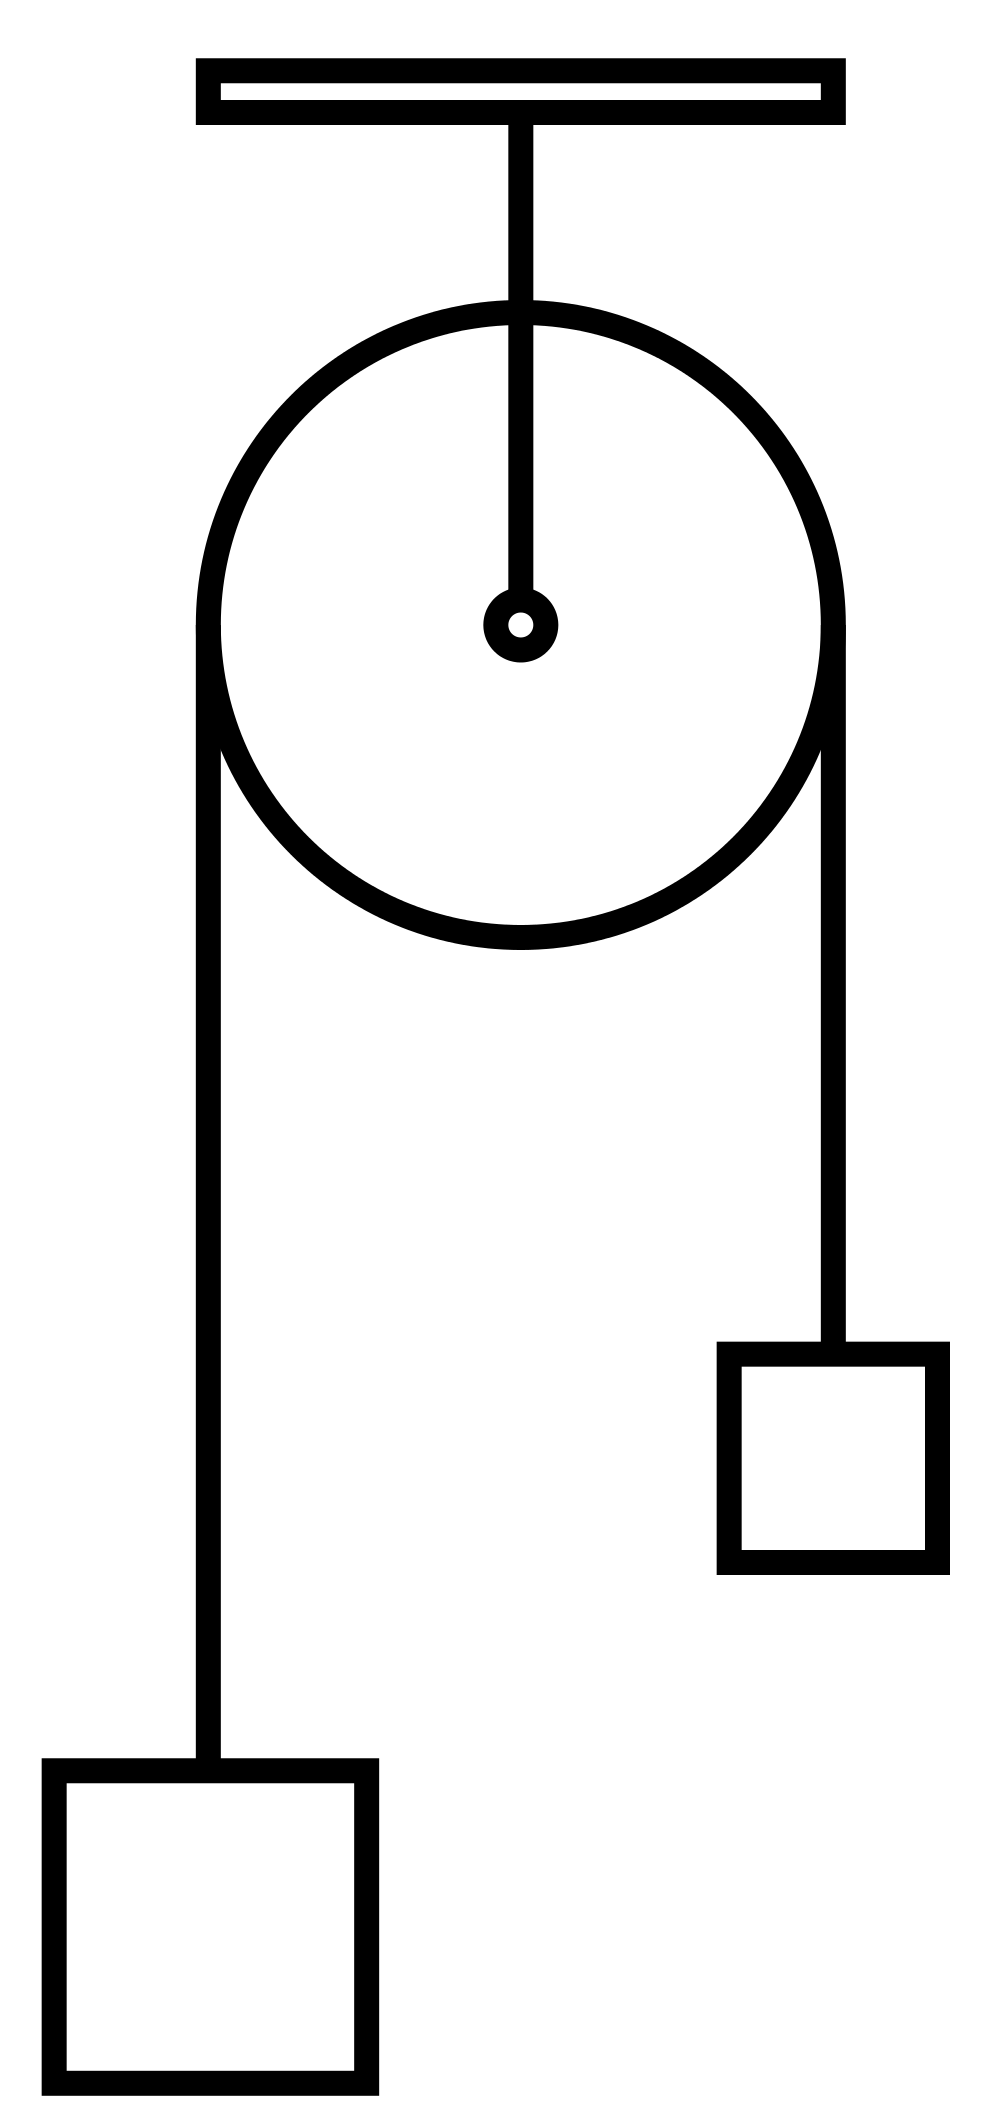
\includegraphics[width=0.5\textwidth]{atwood.png}
\end{center}
\end{minipage} \hfill

a) What do you expect the system to do if one of the masses is much heavier than the other?

\vspace{1in}

b) Draw force diagrams for both objects. Label your choice of coordinate system separately for each object -- you don't have to choose the same coordinate system for each!

\vspace{2in}

c) State Newton's law for both objects. Note that their accelerations aren't necessarily the same, depending on your choice of coordinate system, so you should introduce separate variables $a_1$ and $a_2$ for both. The tension forces
{\it are} the same.

\newpage

d) Since you have two objects, you have two copies of Newton's law. However, you have three unknowns: $T$, $a_1$, and $a_2$. What other statement can you make about the accelerations that lets you solve the system?

\vspace{3in}

e) Actually solve the system, giving values of $a_1$ and $a_2$ in terms of $m_1$, $m_2$, and $g$. What is the acceleration if one mass is twice as big as the other? Does this make sense? 

\newpage

A stack of two books, each of mass 1 kg, sits on a table. The coefficients of static friction between the books, and between the bottom book and the table, are 0.4; the coefficients of kinetic friction are 0.2. A person exerts a sudden force on the bottom book. Intuitively, we know what happens:
\begin{itemize}
\item{I. If this force is moderate, then the two books accelerate together at the same rate.}
\item{II. If this force is very large, then the bottom book is yanked out from beneath the top one, and they accelerate at different rates.}
\end{itemize}

a) In case I, what type of friction exists between the bottom book and the table? What about between the two books?

\vspace{0.7in}

b) In case II, what type of friction exists between the bottom book and the table? What about between the two books?

\vspace{0.7in}

c) Draw force diagrams for the situation when the force is almost large enough to pull the bottom book out from underneath the top one.

\vspace{1.5in}

d) Calculate how much force is required to do this.


\newpage

\centerline{\it \small (This problem and the following one are for Friday)}

  A person uses a rope to spin a bucket in a vertical circle at a constant speed; the radius of the circle is 80 cm. The bucket goes around the circle once every second. Inside the bucket is a friendly frog, happy to be out of the elevator, of mass 500g.


a) Draw a force diagram for the frog when the bucket is at the top of the circle, and when it is at the bottom.

\vspace{2in}

b) What is the acceleration of the bucket?

\vspace{1in}


c) As you saw last week in your homework, your ``apparent weight'' is simply the magnitude of the normal force that an object under you exerts on you. What is the frog's apparent weight at the bottom and at the top of the circle?

\vspace{2in}
\newpage
d) Explain why the frog doesn't fall out of the bucket at the top of the swing, despite the fact that the only forces acting on it point downward.

\vspace{4in}

e) Now, imagine that the person swinging the bucket slows down gradually. At some point, the frog will fall out of the bucket. (It's a frog, so it'll land on its feet and not be hurt!) How low can $\omega$ become before the frog falls out of the bucket?

\newpage


A highway curve has a radius of curvature of 500 meters; that is, it is a segment of a circle whose radius is 500 m. It is banked so that traffic moving at 30 m/s can travel
  around the curve without needing any help from friction.


a) Draw a force diagram for a car traveling around this curve at a constant speed. Draw the diagram so that you are looking at the rear of the car. {\it Hint:} Do not tilt your coordinate axes for this problem!


\vspace{2in}

b) What is the acceleration of the car in the $x-$direction? What about the $y-$direction?

\vspace{1in}

c) Write down two copies of Newton's second law in the $x-$ and $y-$directions.

\vspace{1.5in}

d) Solve the resulting system of two equations to determine the banking angle of the curve.

\end{document}
